
\section{Knowledge Management}
\label{sec:km}

Software development is inherently a knowledge-intensive activity. Software
designers and developers leverage their software-development skills, along with
domain knowledge, past experiences, and the knowledge of team members, to solve
the problem at hand, such as implementing a new feature or resolving a bug.  In
small, collocated teams, knowledge management is not a big challenge---people's
expertise on different parts of a system is typically known. New team members
can use informal communication channels to identify experts and seek their help
as needed.

However, as teams increase in size or become geographically distributed,
knowledge management starts to become challenging. In large or distributed
teams, system knowledge---\eg expertise, dependencies, best practices---is
spread across multiple people, locations, and (in the case of outsourcing) even
organizations~\cite{Desouza:2006}. In such projects, a knowledge-management
system is needed to create \textit{project memories} that can serve different
needs. First, it should assist new team members in understanding the project
with little or no face-to-face guidance and identifying experts to reach out to
for questions. Second, the system should help existing team members identify the
artifacts relevant, and the people they might need to coordinate with, for
performing a task. Existing attempts at creating such project memories include
Hipikat~\cite{Murphy:2005} and Codebook~\cite{Begel:2010}.

A service company has a large, geographically distributed employee base, with
frequent employee churn at project and organization levels. To maintain
consistent delivery quality, it is essential to manage knowledge at the project
level. Moreover, because services is a price-sensitive business, there is also
the need to be cheaper and better, by doing more with fewer or less-skilled
resources. Driven by this need to gain competitive advantage in increasingly
competitive markets, it becomes essential for companies to build
\textit{organization memories} that store the collective knowledge of past
engagements, processes, and people to increase productivity and reduce
activities that ``reinvent the wheel.'' The intent behind such a system is to
ensure that the knowledge of past or current employees is available to other
employees when the need arises. Thus, the organization should be able to
leverage learning and solutions from past client engagements in the context of a
new similar engagement, even when members from the past projects are not around.

The need for organization-level knowledge bases is well established in the
management literature~\cite{davenport2000working,bollinger2001managing}. Equally
well known is the fact that creating an effective organization-wide knowledge
base is very challenging~\cite{McKinsey:1999,Harvard:1999,Ernst:1997}. There are
challenges in: (1) \textit{knowledge creation}---how to codify explicit and
tacit knowledge and motivate individuals to contribute; (2) \textit{knowledge
  retrieval}---data versus information versus knowledge; (3) \textit{knowledge
  governance}---legitimacy, relevance, and quality of contributed
knowledge. Alavi and Leidner~\cite{Alavi:2001} present a good overview of
research issues in organization knowledge management. Prior research suggests
that IT is incapable of capturing organizational knowledge
\cite{malhotra2004knowledge,mcdermott2000information}, but also postulates that
IT is the strongest enabler for organization knowledge management systems
(OKMS).

Next, we present three scenarios illustrating the need for OKMS in service
companies. Then, we discuss promising research directions based on our
experience with building systems intended to promote knowledge reuse in these
scenarios.

\subsection{Scenarios for OKMS}

In this section, we present three typical scenarios in service delivery that can
benefit from an organization knowledge management system.

\subsubsection{Troubleshooting}

One of the common forms of service engagements is application maintenance, where
the expectation from the service provider is to take over a client's custom
application and handle service requests for it.  Service requests come in the
form of trouble ``tickets'': users of the applications can raise a ticket,
logging a problem they have experienced. This is similar to defect logging in
bug repositories, such as Bugzilla, where users of an open-source software can
enter the details of a problem that they encountered.  The main difference is
that, in typical software development in open-source communities, there is no
obligation on the development team to address the defects in a timely
fashion. Likewise, even in a product setting, the development team can
prioritize which defects they are going to address first.  In service context,
the service provider is supposed to resolve the ticket in a timely manner, often
under a service-level agreement. For example, a critical bug must be resolved
within 6~hours, at risk of financial consequences for the provider.

Software development in service organizations is not pure custom
implementations. In many cases, packaged applications, such as SAP, Oracle, and
COTS products, with client-specific customizations and external libraries are
used. The cause of a problem ticket could be in the customization done for the
client, in the way external code is used, or even a bug in the external code. If
the issue is with the configuration or the external code, it is very likely that
the same (or a similar) issue has been resolved previously in the context of
another client. Thus, if the person attempting to resolve the current ticket had
access to previously resolved tickets addressing similar problems, they could be
much more efficient and effective at their task.  Therefore, a knowledge base
that stores past resolved tickets across clients would be a useful
organization-wide resource. 

In a way, such a knowledge base would be similar to public question-and-answer
forums we see on various software languages, tools, and open-source projects on
the web.

\subsubsection{Design-build Projects}

Another common form of service engagement is business-process transformation,
where the expectation from the service provider is to IT-enable a business
process, such as payroll management, vendor management, order-to-cash, for a
client. Some business processes (\eg payroll management) would be required by
all clients, whereas other processes would be common in a particular domain (\eg
claim-management process in the insurance domain).  The client expectation is
that the service provider possesses adequate knowledge of the generic version of
a particular process, creates client-specific variations, and implements the
system. Typically, this requires that the vendor team working on the project has
significant domain experience.

A knowledge-management system that stores past business process implementations
across the organization can help in this scenario. The past solutions need to be
organized by domain to make retrieval of relevant information
easier. Appropriate documentation that explains the standard and customized
portions of past solutions needs to be available, along with the solution
code. While designing a new business-process solution, the team can search
through the repository to learn about the variations of the process to be
implemented and, if the client requirements are not too different from a past
solution, even reuse the solution in totality or parts. This can reduce the
overall cost and also potentially let the service provider staff the team with
people with less domain experience. 

Code reuse, at different levels of granularity---lines-of-code level, API level,
and even complete solutions---has been an area of interest in the
software-engineering community~\cite{Reiss:2009,Holmes:2013}. Much of this work
could be applied in the setting of a service company too.

\subsubsection{Service Improvement}

When a client outsources its application maintanence to another organization,
one of the key expectations is that the vendor would bring down their total cost
of ownership over time. This requires the vendor to proactively seek out areas
for improvement in the client application portfolio. One way to determine
whether there is scope of improvement in an application in the client IT
landscape is by benchmarking its performance against other similar applications
in other client landscapes. To illustrate, suppose that a service company
maintains the payroll applications for 10~clients. For nine of the clients, the
monthly ticket volumes range between 5 and 10 tickets, whereas, for the
remaining client (say client~A), the ticket volume ranges from 20 to 50. This
indicates that, for client~A, investigations could be conducted to determine the
root causes for high ticket volumes and appropriate preventive actions
taken. Moreover, if a similar high-ticket-volume problem was seen in the past in
another client's payroll system, information about the actions taken for that
client could help the team resolve the problem for client~A.

There are a number of organizations that gather and report quantitative
benchmark information (qualitiative as well as productivity) for software
projects and business applications depending on language used to code, number of
users etc. CAST, Software Engineering Institute are some examples of such
organizations. However, considering services organizations are doing multiple
software implementations for multiple clients, an organization-wide knowledge
base that (1) captures key operational metrics per application (or at a more
granular level, such as by problem area) per client and the past improvement
actions taken, and (2) allows comparisons between clients with similar
applications and problems encountered, would help augment what is publicly
available and be more useful.

\begin{figure*}
	\center
	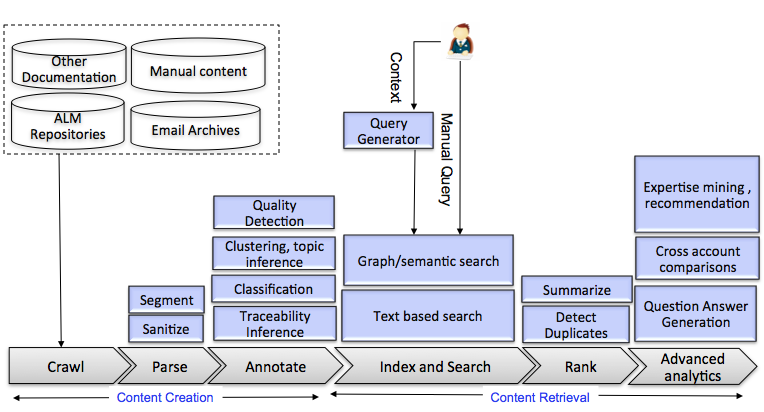
\includegraphics[scale=0.45]{figs/km.png}
        \vspace*{-10pt}
	\caption{System architecture for an OKMS system for a service company.}
        \vspace*{-10pt}
	\label{fig-km}
\end{figure*}

\subsection{Research Topics}

Based on such OKMS needs in IBM's service-delivery organization, there have been
efforts toward implementing systems to address the needs. These include a system
for promoting solution reuse in design-build engagements centered around
business-process transformation~\cite{Goodwin:2012b}, and a system that enables
cross-account sharing of knowledge in problem tickets~\cite{Majumdar:2011}.

We now discuss some core problems that need to be addressed in creating OKMS in
service organizations. At the simplest level, an OKMS is a database where
content can be stored and retrieved from. However, what content should be
stored, how easily can the content be stored, and the ease with which relevant
content can be retrieved determines the usefulness of an OKMS.
Figure~\ref{fig-km} presents the general architecture for an OKMS in services,
which we use to highlight the activities performed and the related topics (shown
in the boxes) that would benefit from further research. 


\subsubsection{Knowledge Creation}

What constitutes useful knowledge in a service company? How can such knowledge
be collected and organized? These are some of the questions that need to be
addressed in knowledge creation. Specifically, we discuss three aspects of
knowledge creation: \textit{crawling}, to collect content from diverse
sources; \textit{parsing}, to translate the content in various formats into a
standard format; and \textit{annotating}, to extract metadata from the content
that can help organize it.

\vskip -5pt
\paragraph*{Crawling} The first activity in building an OKMS is
identifying the data that should be stored in the repository and how to obtain
the data. In general, this activity includes a combination of manually provided
data and automatically crawled data, each of which can have its own peculiar
challenges.

For manual data collection, an organization can require its employees to
contribute learnings and software artifacts to the OKMS. For instance, this
could be done via FAQs, where employees outline solutions to common problem
tickets they have resolved; or, it could be done via postmortem reports, usage
stories, and experience reports~\cite{desouza:2005} created by project members
after the resolution of a key project issue. If a client solution involves
software development, employees can be asked to identify reusable software
components and contribute them, after generalization, to the OKMS.

Manual content creation puts extra burden on the employees, beyond their normal
delivery-related responsibilities. Thus, an interesting problem is how to
motivate employees to contribute high-quality content to the
OKMS~\cite{hendriks1999share}. Incentive mechanisms could include ``badges'' as
is done in open-source forums, such as stack exchange to encourage question and
answer contributions. In a service company, would reputation-building incentives
be sufficient or would monetary or career-growth incentives be
necessary~\cite{bartol2002encouraging}?

%% An organization has the option of mandating that each of it's employees
%% contributes their learnings to the OKMS system. Some examples of manual
%% knowledge creations are: (1) frequently asked question, where employee outlines
%% the typical solutions to some common problem tickets they have resolved (2)
%% postmortem reports, usage stories, experience reports\cite{desouza:2005}, that
%% project members can create after they solve a key issue in the project. To
%% enable solution reuse, services organizations often invest in creating software
%% product families
%% \cite{clements2002software}. However, here it's pre-anticipated what could be
%% some solutions that could be of interest to multiple clients in a particular
%% domain such as healthcare and then those solutions are created with appropriate
%% points for variability built in, so solution can be customized for any client
%% intending to use it.  Once a project is completed, employees are also encouraged
%% to identify reusable components in software they created and share them in the
%% knowledge base. This approach of manual content creation adds extra burden on
%% the employees. An open research challenge is to motivate employees to contribute
%% high quality content in the knowledge base \cite{hendriks1999share}. Open source
%% forums such as stack exchange have experimented with elaborate incentive
%% mechanisms in forms of badges to ensure questions and answer contributions on
%% their forums \cite{vasilescu2014social}. In services organizations are
%% reputation building incentives enough or incentives should translate to monetory
%% benefits and/or career progression /cite{bartol2002encouraging}?

In addition, or as an alternative, to manual content creation, content can be
collected through automated crawling of the artifacts produced in a project. For
example, complete traceability from requirements through code to test cases,
along with relevant content, can be extracted from Application Lifecycle
Management tools. Similarly, information about problem tickets and their
resolutions can be extracted from ticket-management systems.  Account teams
periodically report important metrics, such as ticket volumes, code changes, and
service-improvement actions taken, on the client applications being maintained;
these reports could be automatically pushed into the OKMS. The main challenge
here is extraction of this data from the diversity of tools and technologies used to create software
artifacts and related information across projects.

%% Another approach for content creation is to auto-harvest artifacts produced in
%% the SDLC lifecycle and put these in the knowledge management system. Complete
%% traceability from requirement through code to test cases, along with their
%% content is extractable from Application Lifecycle Management tools and this can
%% act as solution packs to put in the repository. Similarly for ticket resolution,
%% information about problem ticket and it's resolution is extractable from ticket
%% management systems. Account teams periodically report on various important
%% metrics on the applications being maintained in the client landscape such as
%% ticket volumes, code changes, service improvement actions taken. These reports
%% can be auto pushed into the knowledge repository. The main challenge here is
%% handling the diversity of tools and technologies used to create SDLC data across
%% projects.

\vskip -5pt
\paragraph*{Parsing} After data has been pulled from various
sources, the next activity involves parsing different document formats and
templates into a standardized format that can be pushed into the knowledge
repository. The diversity of formats, some of which may be proprietary, makes
automated content parsing a challenging problem and a fruitful research
direction. For instance, a possible approach could be based on writing
model-to-model transforms~\cite{debdoot:2010:scc}.

Another issue is that the traceability information necessary for understanding
the context of how and why an artifact was produced might be missing---for
instance, traceability between code commits and bug reports is necessary to support knowledge reuse for troubleshooting. Similarly, traceability between requirements and application code is desired to enable reuse of business process software implementations across projects. The gaps in traceability  occur
primarily due to lack of integration between the tools used to create the
artifacts. In such cases, automated analyses must be developed for inferring the
traceability; this is an active area of research~\cite{spanoudakis2005software},
with different types of approaches, such as those based on information
retrieval, traceability rules, special integrators, and inference axioms, being
developed.

%% \paragraph*{Parsing} Once all the requisite data has been pulled from various
%% sources, the main challenge is parsing of the data from various document formats
%% and templates into a standardized format that can be pushed into the knowledge
%% repository. Many of the crawled data is in form of documents in proprietery
%% formats such as Microsoft word, power point slides, visio diagrams, excel
%% sheets. How to automate content extraction from client specific work products
%% into the standard format used by knowledge repository is again a direction for
%% research. One approach is to write model to model transforms where a project
%% admin can specify the mapping \cite{debdoot:2010:scc}. Another challenge is that
%% requisite traceability information that is required to understand complete
%% context of how and why an artifact was produced, might be missing. This is
%% because tools being used to create different SDLC artifacts have not been
%% integrated. There is need to auto infer traceability between artifacts For
%% example, if making a code commit, the developer puts in a comment like "Fixed
%% Bug \#145", then with high confidence the change is to fix "Bug \#145" and
%% traceability edge between code file and bug report should be auto-created.
%% . Tracability inference is an active area of
%% research \cite{spanoudakis2005software}. Some proposed approaches use
%% information retrieval (IR) techniques, others use traceability rules, special
%% integrators, and inference axioms.

In service delivery, the OKMS is populated with data collected at client
engagements and can include client-confidential and sensitive information (\eg a
problem ticket might contain the contact information of the user). Thus, a
critical requirement for the OKMS, which would benefit from automation, is
cleansing or anonymization of all sensitive and client-confidential information.

%% The content in a OKMS database comes from various clients:. There are strict
%% privacy constraints around what data is client confidential and hence cannot be
%% shared. Within a single artifact itself, there might be small portions of
%% content that are client confidential. E.g. a problem ticket might content the
%% contact information of the user who encountered the information. How to remove
%% client confidential data from artifacts put in the repository, how to anonimize
%% the content so as to not disclose client identity and how to ensure that only
%% authorized users and roles have access.

\vskip -5pt
\paragraph*{Annotating}
The content in the OKMS must be organized for easy retrieval. The general
practice to do this is to classify OKMS content against predefined
taxonomies. For example, a simple taxonomy is the artifact type: requirement,
code, problem ticket, etc. More generally, a taxonomy ought to include
information about industry type and process area~\cite{apqc,bph}, technologies
used, etc. Organizations spend effort in building and maintaining these
taxonomies; automated tool support to assist with this would be useful. For
instance, clustering~\cite{Berkhin06} and topic-modeling
techniques~\cite{Blei:2012} could be leveraged to group similar content and
infer topics from them.

Manual classification of data can be tedious and prone to human errors. To
reduce this effort, automation via pattern matching and machine-learning-based
classification approaches~\cite{bishop2006pattern} could be used.  The
effectiveness of these techniques depends on the availability of positive and
negative samples to train a learning model. Often, due to unavailability of
training data and/or lack of differentiating features, usual learning techniques
such as na\"{\i}ve bayes, support vector machines, and decision
trees, do not attain sufficient precision and recall. Thus, there is a
need to customize more advanced learning approaches (\eg
ensemble techniques~\cite{Dietterich:2000}) or develop new techniques that are more effective
on the typical data available in service delivery.

%% One taxonomy is obviously the object type i.e. requirement, code,
%% problem ticket (further segmented into problem description, resolution). Another
%% taxonomy captures the domain the artifact was produced in i.e. industry type and
%% process area e.g. \cite{apqc,bph}. Another taxonomy is the technology
%% used. Organizations spend effort building and maintaining these taxonomies. For
%% every data that is put into the knowledge base, the content needs to be manually
%% categorized against these pre-defined taxonomies. Pattern matching and machine
%% learning based classification approaches /cite{bishop2006pattern} can be used to
%% auto-categorize content to these pre-defined taxonomies. These techniques rely
%% on the availability of equal proportion of positive and negative samples to
%% train a learning model. However, due to unavailability of training data and/or
%% lack of differentiating features, usual learning techniques such as naive bayes,
%% support vector machines, decision trees, might end up not giving desired
%% efficacy (measured as precision and recall). There is need to customize more
%% advanced learning approaches such as adaptive learning, ensemble techniques or
%% develop new techniques that work well with SDLC data. Another interesting area
%% for research is to explore how to help grow the taxonomy over time based on
%% content coming in the knowledge base. Techniques such as
%% clustering \cite{Berkhin06}, topic modeling \cite{Blei:2012} help group together
%% similar looking content and infer topics out of them.


The data in an OKMS can quickly grow very large. For example, in just a year, a
problem ticket repository we setup in IBM grew to contain 750,000 tickets;
similarly, our business process solution repository~\cite{Goodwin:2012b}
contains approximately 16,000 solutions. Given this scale, ensuring high quality
of the data (\eg filtering out non-reusable content) is challenging but
essential. Different approaches could be followed for ensuring data quality,
such as human vetting of incoming OKMS content or based on human feedback on
usefulness of retrieved content. An interesting research direction would be to
explore automatic quality scoring of artifacts, taking into consideration
technical and non-technical artifact content, reputation of artifact authors,
etc. For example, such approaches have been investigated
in~\cite{Majumdar:2011}.

%% Once an OKMS system is implemented in an organization, irrespective of the
%% approach to collect content i.e. manual, automated harvesting or hybrid, the
%% repository starts filling up fast. Over a period of one year, the problem ticket
%% repository we setup within IBM collected 750K tickets. Similarly, the business
%% process solution repository has 16000 solutions. However, not all content being
%% put in the repository is high quality and reusable. Hence, it is becomes
%% imperative to be able to filter out useless content. One way to achieve this is
%% by making a human vet every content being pushed in the repository and only
%% content that is deemed high quality is published. Another approach is to ask
%% people who are retrieving and potentially using the content, give feedback on
%% whether they found content useful or not. The third approach that makes for an
%% interesting research direction is to explore how a an automatic quality score
%% can be assiged to each artifact based on content in the artifact, prior
%% reputation of people who authored the content, whether the project was a success
%% or not and so on. In our problem ticket repository, we experimented with
%% calculating a quality score per ticket based on technical versus non-technical
%% content present in the ticket \cite{Majumdar:2011}.


%% \paragraph*{Summary} To summarize, content creation in OKMS provides multiple
%% oppurtunities where research can contribute. These include: what and how to
%% extract content from SDLC repositories and proprietry document formats, how to
%% infer traceability between different artifacts, how to classify and categorize
%% content, how to maintain privacy, estimate quality and motivate employees to
%% contribute high quality content.


\vspace{-5pt}
\subsubsection{Knowledge Retrieval}

Challenges in knowledge retrieval are related to the search capabilities offered
by the OKMS and the effort required from users in determining the usefulness of
the recommended data. We discuss the following aspects of knowledge retrieval:
indexing and searching, search result organization, and advanced analytics.

\vskip -5pt
\paragraph*{Indexing and Searching} The simplest approach for searching
is \textit{keyword-based search}, in which users specify the words they are
looking for and the system returns all artifacts that contain the specified
words. More sophisticated systems use \textit{faceted search}, where the user
can navigate a hierarchical structure (\eg a taxonomy) and select values from
predefined categories.  Despite the availability of many search technologies,
studies such as \cite{idc2}) have shown that retrieval of relevant information
from organizational repositories remains challenging, with users being
successful in less than 50\% of their attempts in searching for information.

Language-based information-retrieval techniques~\cite{manning2008introduction},
on which many knowledge systems are based, may be inadequate in dealing with the
types of repositories we are talking about---that contain not just a collection
of artifacts, but a network of linked artifacts.  Graph databases for storage
and semantic search techniques~\cite{Guha:2003} or extending keyword search for
graphs~\cite{kacholia2005bidirectional} may be more promising in this scenario,
and are worthy of research investigation.

%% \paragraph*{Index and Search} Indexing is how the knowledge repository stores
%% data internally. Search features then work on this index.  Typical ways to
%% retrieve content from a knowledge base are: (1) keyword based search where user
%% specifies a couple of words (s)he is looking for and all artifacts in the
%% repository that contain the words from user query are returned, (2) faceted (or
%% navigational) search where user is shown a hierarchy structure (taxonomy) and
%% can browse information by choosing one or more values from each of the
%% pre-defined categories. Various language based information retrieval
%% models \cite{manning2008introduction} such as vector space models, probablistic
%% models, latent semantic index exist that can be used here. But inspite of easy
%% to use search technologies being available, prior studies report that knowledge
%% retrieval from organization wide repositories remains a challenge. As
%% per \cite{idc,idc2}, while employees spend 15\% to 35\% of their time searching
%% for information in an enterprise, they are successful less than 50\% of the time
%% in finding what they are looking for. Most existing OKMS systems use language
%% based IR models to store and retrieve knowledge. However, as we saw in content
%% creation section, the repository is not just a collection of artifacts but a
%% network of linked artifacts. Use of graph databases for data storage and
%% retrieval techniques such as semantic search techniques \cite{Guha:2003} or
%% optimizing keyword search for graphs \cite{kacholia2005bidirectional}, are worth
%% exploring.

An important factor in performing accurate search is the expressiveness of query
construction. Simple keyword queries, consisting of a set of words, may not be
discriminative enough to return accurate results. A few approaches have been
developed to address this problem, for example, by giving more weights to words
that appear in the title of a problem ticket than words that appear in the
ticket description~\cite{Sinha:2012}, and using separate queries for different
types of information, such as description, application information, and stack
trace, in a problem ticket~\cite{Ashok:2009}.

Another question pertains to assigning weights to clauses in the query while
ranking the search results~\cite{Debdoot:2011:bpm}. Moreover, the idea
of \textit{contextual search}~\cite{wen2004probabilistic,kraft2005q}, which
attempts to capture the user's information needs better by augmenting the query
with contextual information extracted from search context, has shown promising
results. Further research along these directions---in the context of the
knowledge needs in service delivery---investigating different ways of creating
contexts, using contexts in constructing queries, and assigning weights to query
clauses would be interesting.

%% Non-availability of content or poorly organized content can be one reason for
%% this. Another reason could be the inadequacy of the query itself that are used
%% to retrive the content. Suppose a user is trying to find problem tickets that
%% resolved similar issues to what (s)he has been assigned. (S)he would pick up a
%% couple of words from the ticket that describe the problem and use it to query
%% the knowledge base. However, these words might not be discriminative enough and
%% user might end up getting too many or too little search hits. Another approach
%% could be to use complete content in the ticket and use it as query. However in
%% this case, the search engine might end up returning irrelevant results as equal
%% weightage was given to all words in the problem ticket. \cite{Sinha:2012} tries
%% to address this issue by giving more weightage to those words in the query that
%% belong to ticket title. \cite{Ashok:2009} parses out different datatypes from a
%% problem ticket such as description, application information, stack trace and
%% using a different query/search mechanism for each. E.g. instead of just
%% specifying "null pointer exception", the query generated from a problem ticket
%% could be---description: contains following bag of words \{null, pointer,
%% exception\}, process: is equal to "order to cash", stack trace: contains
%% foo.*bar. The results obtained from such a query are likely to be more precise
%% than what a keyword search would yield. A challenge with this approach is how to
%% compose the various clauses in the query---are they "anded" or "ored" or a
%% combination. Another challenge is how much weightage to give to each clause when
%% ranking the search results \cite{Debdoot:2011:bpm}. Moreover, recently
%% contextual search \cite{wen2004probabilistic,kraft2005q} has been gaining
%% momentum. Contextual search tries to better capture a user's information need by
%% augmenting the query with contextual information extracted from search
%% context. It would be an interesting direction for future research to see for
%% each of the knowledge needs in services organizations, what can make up the
%% context, how to use this context to create the query and how to weigh different
%% clauses in the query.

\vskip -5pt
\paragraph*{Search Result Organization}
Although more powerful querying capabilities can help improve the accuracy of
search results, a search-based system would in general return multiple
results. The next question then is: how much effort does it take for the user to
sift through the results to find relevant information? Simple approaches such as
highlighting matching keywords will not work for complex queries; more
sophisticated techniques that help the user easily comprehend the relevance of
the results are needed. One such approach is \textit{summarization}, which has
been used in text-processing domains to end users get a quick overview of
information; summarization has also been applied to bug
reports~\cite{Mani:2012,Rastkar:2010}. Extending this notion to other types of
artifacts, such as code, requirements, and solution designs, is an open topic
for research.

Another type of analysis that can improve the search results is detection and
grouping of duplicates or near-duplicates. By grouping together such artifacts
and highlighting the variances in seemingly similar artifacts, the system can
reduce information overload on the user.  Detection of duplicate bug reports has
been widely researched
(\eg \cite{wang2008approach,sun2010discriminative}). Developing such analyses
for other types of artifacts, from a services OKMS perspective, would be useful.

Typically, an OKMS would display the search results as a ranked list, with
10--20 items per page. The ranking can be based on relevance of artifacts,
quality of artifacts, past user ratings given to artifacts, etc. Prior research
have explored other novel ways to visualize search results
(\eg \cite{Nowell:1996,Shneiderman:2000}).  Another potential direction for
research is the investigation of effective non-list visualizations of OKMS
artifacts.

%% What kinds of non-list visualization
%% would be effective in organization knowledge management system that are
%% predominantly composed of SDLC artifacts is another direction for research.

%% \paragraph*{Search Result Organization}
%% Any search based system would return multiple results. For the user it becomes a
%% chore in itself to go over each of the search results and identify if it is
%% relevant or not. Techniques that can help the user easily comprehend the
%% relevance of the returned results are much needed. Text based search engines
%% highlight the matching words between query and content of the artifact
%% returned. However, when the query becomes complex (as above), keyword
%% highlighting is not of much help. In text processing domain, summarization is
%% one approach that is used to help end users get a quick idea of what the content
%% is about. In \cite{Mani:2012,Rastkar:2010} authors present different techniques
%% to summarize bug reports. Research can help in developing summarization
%% techniques that work for other SDLC artifact such as code, requirements,
%% solution design documents and so on. Further, out of the search results returned
%% many artifacts could be duplicates or near duplicates of each other. In order to
%% reduce information overload for end user, the OKMS system should be able to
%% group together duplicates and near duplicates and be able to highlight the
%% variances in seemingly similar artifacts returned in the search
%% results. Duplicate bug report
%% detection \cite{wang2008approach,sun2010discriminative} has been a widely
%% researched topic. Similarly for each of the artifact of interest from a services
%% OKMS perspective, a customized duplicate detection approach might be needed.

\vskip -5pt
\paragraph*{Advanced Analytics}
Most knowledge-management systems today stop at providing search
capabilities. Given the magnitude of data that can be collected in OKMS, there
is the opportunity of implementing advanced analytics that go beyond by
supporting decision making. Consider the scenario of troubleshooting where, to
resolve a ticket, the user searches through past resolved tickets to find
similar tickets.  Based on the past tickets and the current context, the user
has to formulate potential hypotheses about the root cause, decide which
hypotheses are applicable, and then investigate the solutions. The OKMS would be
much more useful if it could automatically generate potential hypotheses about
root causes and solutions for the user to investigate.

Service requests or tickets contain a lot of information in unstructured text format. Textual analytics applied on this data can help provide useful insights. For example, clustering on service tickets text could help identify problem areas that are causing higher maintanence grief and hence are good candidates for doing preventive work. This approach is discussed in \cite{mani2014}. Analysis of groups of similar problems and resolutions can be used to auto extract out frequently asked question and answers from service requests. In \cite{henss12} authors have presented a text mining and natural language processing based approach to extract FAQs from questions being asked on mailing lists of open source projects.

The effectiveness of knowledge retrieval in the context of service delivery
depends to a large extent on the user's ability to identify projects similar to
the project under consideration. What makes two projects similar? Is it the
technologies being used, the project size, similarity of applications, or a
combination of these and other factors? Investigation of this question and
development of automated techniques for identifying similar projects is needed.

%% \paragraph*{Advanced Analytics}
%% OKMS today stops at providing search capabilities. Given a user query, the
%% system returns back matching artifacts but makes no attempt at making any
%% deductions. Consider the scenario of troubleshooting. A user is searching
%% through the past resolved ticket repository to see if similar issues were
%% resolved. There are multiple reasons why the issues could have arisen. Based on
%% past tickets, the user needs to come up with potential hypothesis of why the
%% issue could be arising and based on conditions (s)he is seeing in the current
%% landscape decide what hypothesis is applicable and then pick the appropriate
%% solution. From such a user's perspective the OKMS system would be more effective
%% if it were able to auto-generate these potential root causes and solutions
%% hypothesis. Consider the service improvement use case, the accout team needs
%% support from OKMS to identify similar projects, then compare the problems seen
%% in the current project with different kind of issues arising in similar
%% projects, then judge whether current team is doing better or worse and then
%% decide to take some action. What kind of capabilities are needed in OKMS system
%% to be useful in above scenarios is another area for research.

%% Much of the knowledge retrieval first requires that user is able to identify
%% similar projects in the organization and then dig deeper into them for learning
%% or comparison with situation at hand. What makes two projects similar? Is it
%% technologies being used or project size or similarity in applications or a
%% combination? Hence, analysis to identify similar projects, compare a project
%% against multiple other projects and auto-summarize similarities and differences
%% is needed.

In general, there are two aspects of organization knowledge management:
codification and personalization~\cite{hansen2000s}. Our discussion of OKMS has
so far focused on the codification aspect, where knowledge is carefully captured
and stored in a knowledge base for use by anyone in the company. The
personalization aspect ties knowledge to specific people; the main purpose of
knowledge management here is to help the user find and connect with people who
have the requisite knowledge, not store the knowledge. This strategy is
especially appropriate in cases where knowledge cannot be easily codified, such
as the knowledge for handling situations that require complex decision
making. Expertise browsing, recommendation, and mining have been explored in
various contexts (\eg \cite{Balog:2006, Mockus:2002}). Extending
these ideas to the context of service delivery, where the OKMS contains data
from multiple projects in different contexts, is an area where further research
can help.

%% There are two techniques for organization knowledge management, codification or
%% personalization \cite{hansen2000s}.  Till now what we have discussed is what is
%% called codification. Here knowledge is carefully captured and stored in the
%% database, where it can be accessed and used by anyone in the company. This
%% strategy allows many people to search for and retrieve knowledge without having
%% to contact the person who originally developed it. This opens up the possibility
%% of achieving required scale in knowledge reuse in services
%% organizations. Another strategy for knowledge management is
%% personalization. Here knowledge is tied to person who developed is and is shared
%% mainly through direct person-to-person contacts. The chief purpose of knowledge
%% management system here is to help people find and connect to other people who
%% have requisite knowledge, not to store it. This strategy works well when
%% knowledge cannot be codified especially knowledge required to handle situations
%% that require complex decision making. Expertise browser \cite{Mockus:2002},
%% expertise recommender \cite{McDonald:2000} have attempted to identify experts on
%% various topics within a project. \cite{Balog:2006} has explored expertise mining
%% and recommendation in predominantly document based OKMS systems. What
%% information to use to mine expertise when repository contains SDLC data from
%% multiple projects, how to match your current context and job profile to suggest
%% people you should have in your network is another scenario where research can
%% help.

%% \paragraph*{Summary} To summarize, content retrieval in OKMS system provides
%% open research problems in query generation and use of context to augment
%% queries, search result summarization, duplicate detection, use of semantic
%% search to improve search relevance. Further the retrieval capabilities need to
%% move beyond just search to provide capabilities such as question-answer
%% generation, cross-account comparison/benchmarking and expertise recommendation.



